\section{Background Prediction and Validation}
\label{sec:BackgroundEstimation}

This section describes the strategies for  the prediction of the background contributions and validation of these predictions.
Monte Carlo  simulation is extensively used to model the kinematic properties of the background and signal processes.
However, since the  simulation of any process is usually prone to systematic
uncertainties due to a non-perfect description of the pileup effects,
underlying event and detector performance, the background contributions from 
$\Ztautau$ and QCD multi-jet process are estimated using dedicated signal-free control data samples, 
as described respectively in section~\ref{sec:ztau} and~\ref{sec:qcd}.
%estimate backgrounds from data. In particular for the following cases:
%\begin{itemize}
%  \item[$\bullet$] The $Z \rightarrow \tau\tau \rightarrow ll ~ + ~  4\nu$ is estimated from data using the embedding technique described in Section~\ref{sec:data_mc}.
%  \item[$\bullet$] The multi-jet background is estimated completely from data using the so-called ABCD method.   
%\end{itemize}
Contributions of other background processes, such as \ttbar, single top quark, dibosons, $Z
\rightarrow ll$ + jets (where $l = e,\mu$) and W + jets, are estimated
from simulation. Given the relatively large \ttbar background contribution, a dedicated study to validate
this background prediction has been made as described in section~\ref{sec:top_est}.

A good agreement between data and background prediction is found after the common selection, as can be seen in 
Figure~\ref{fig:selections} and Figure~\ref{fig:validation}.


\begin{figure}[p]
     \begin{center}
            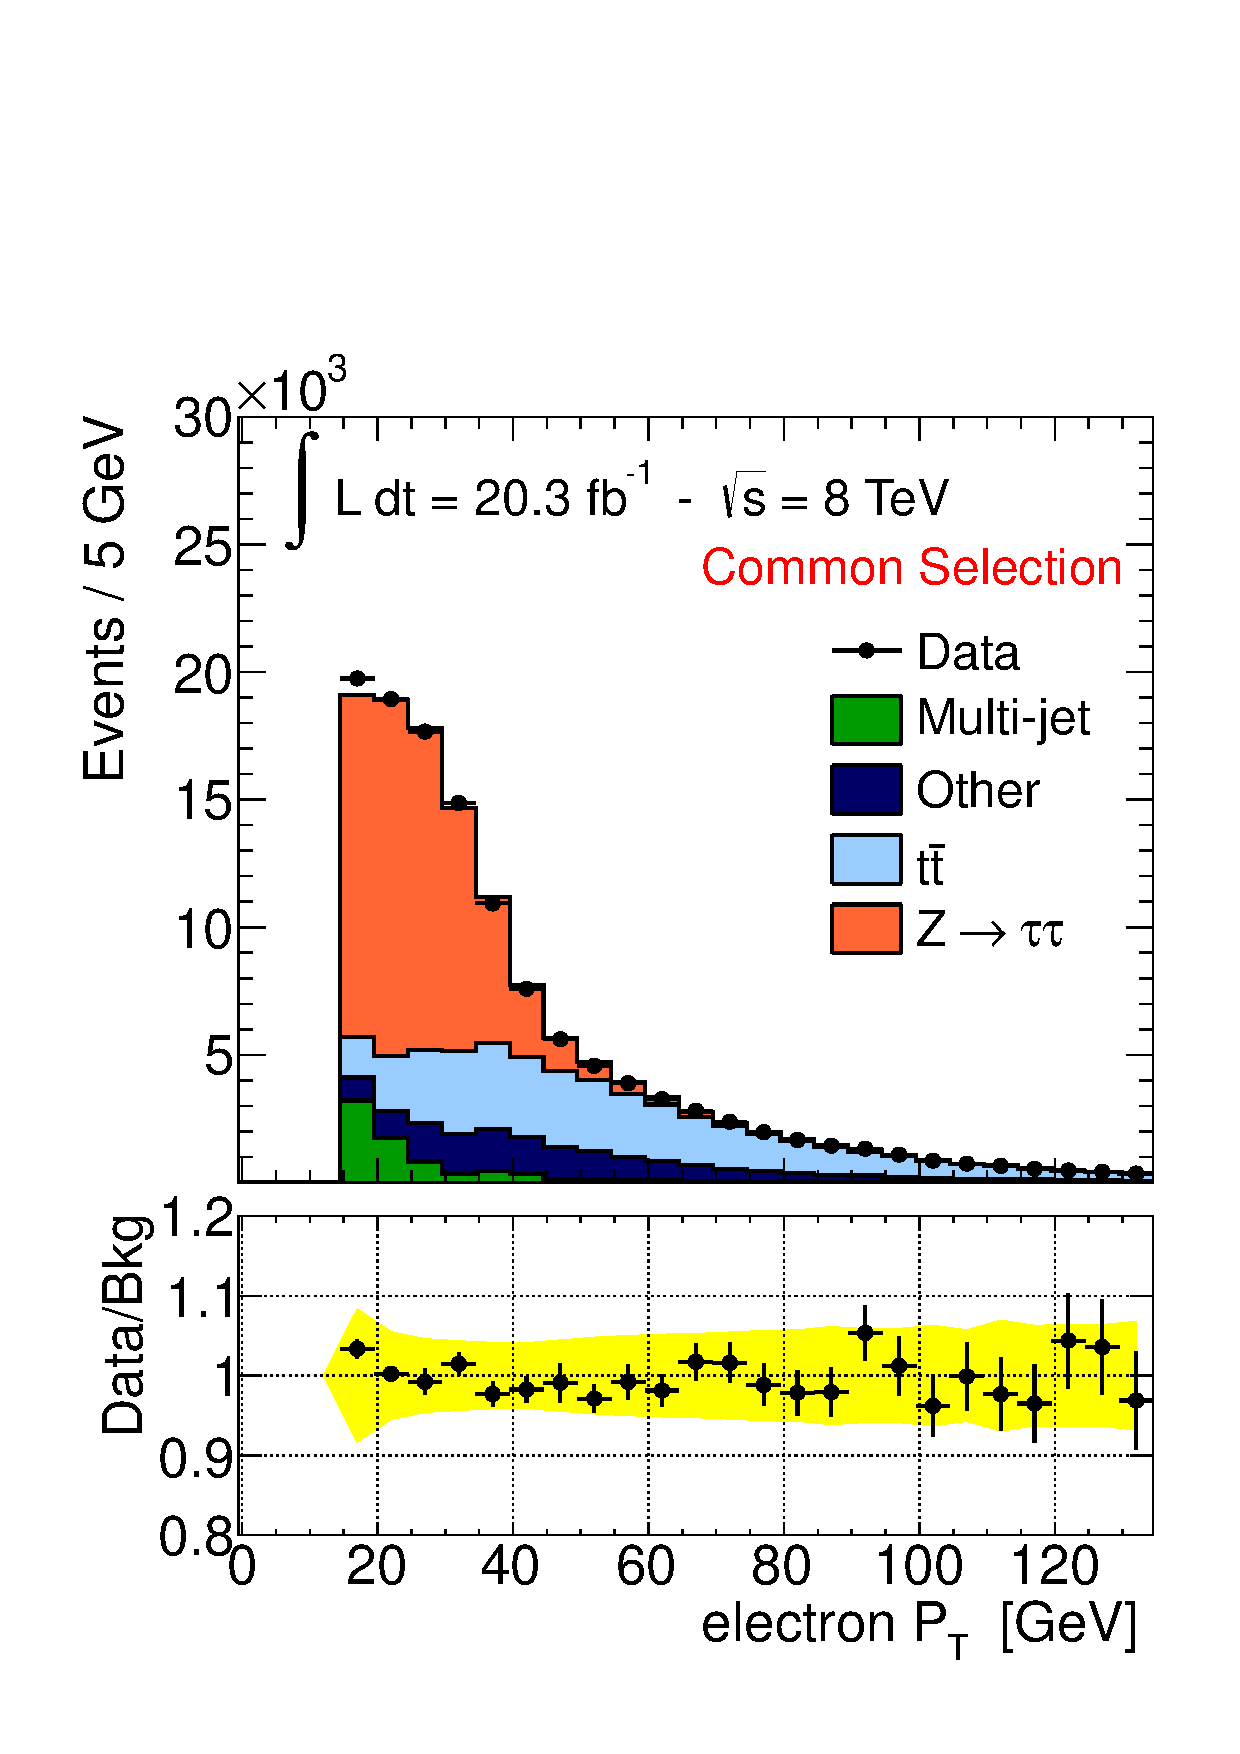
\includegraphics[width=0.47\textwidth]{figure/final_plots/std_presel_ele_pt.pdf}
            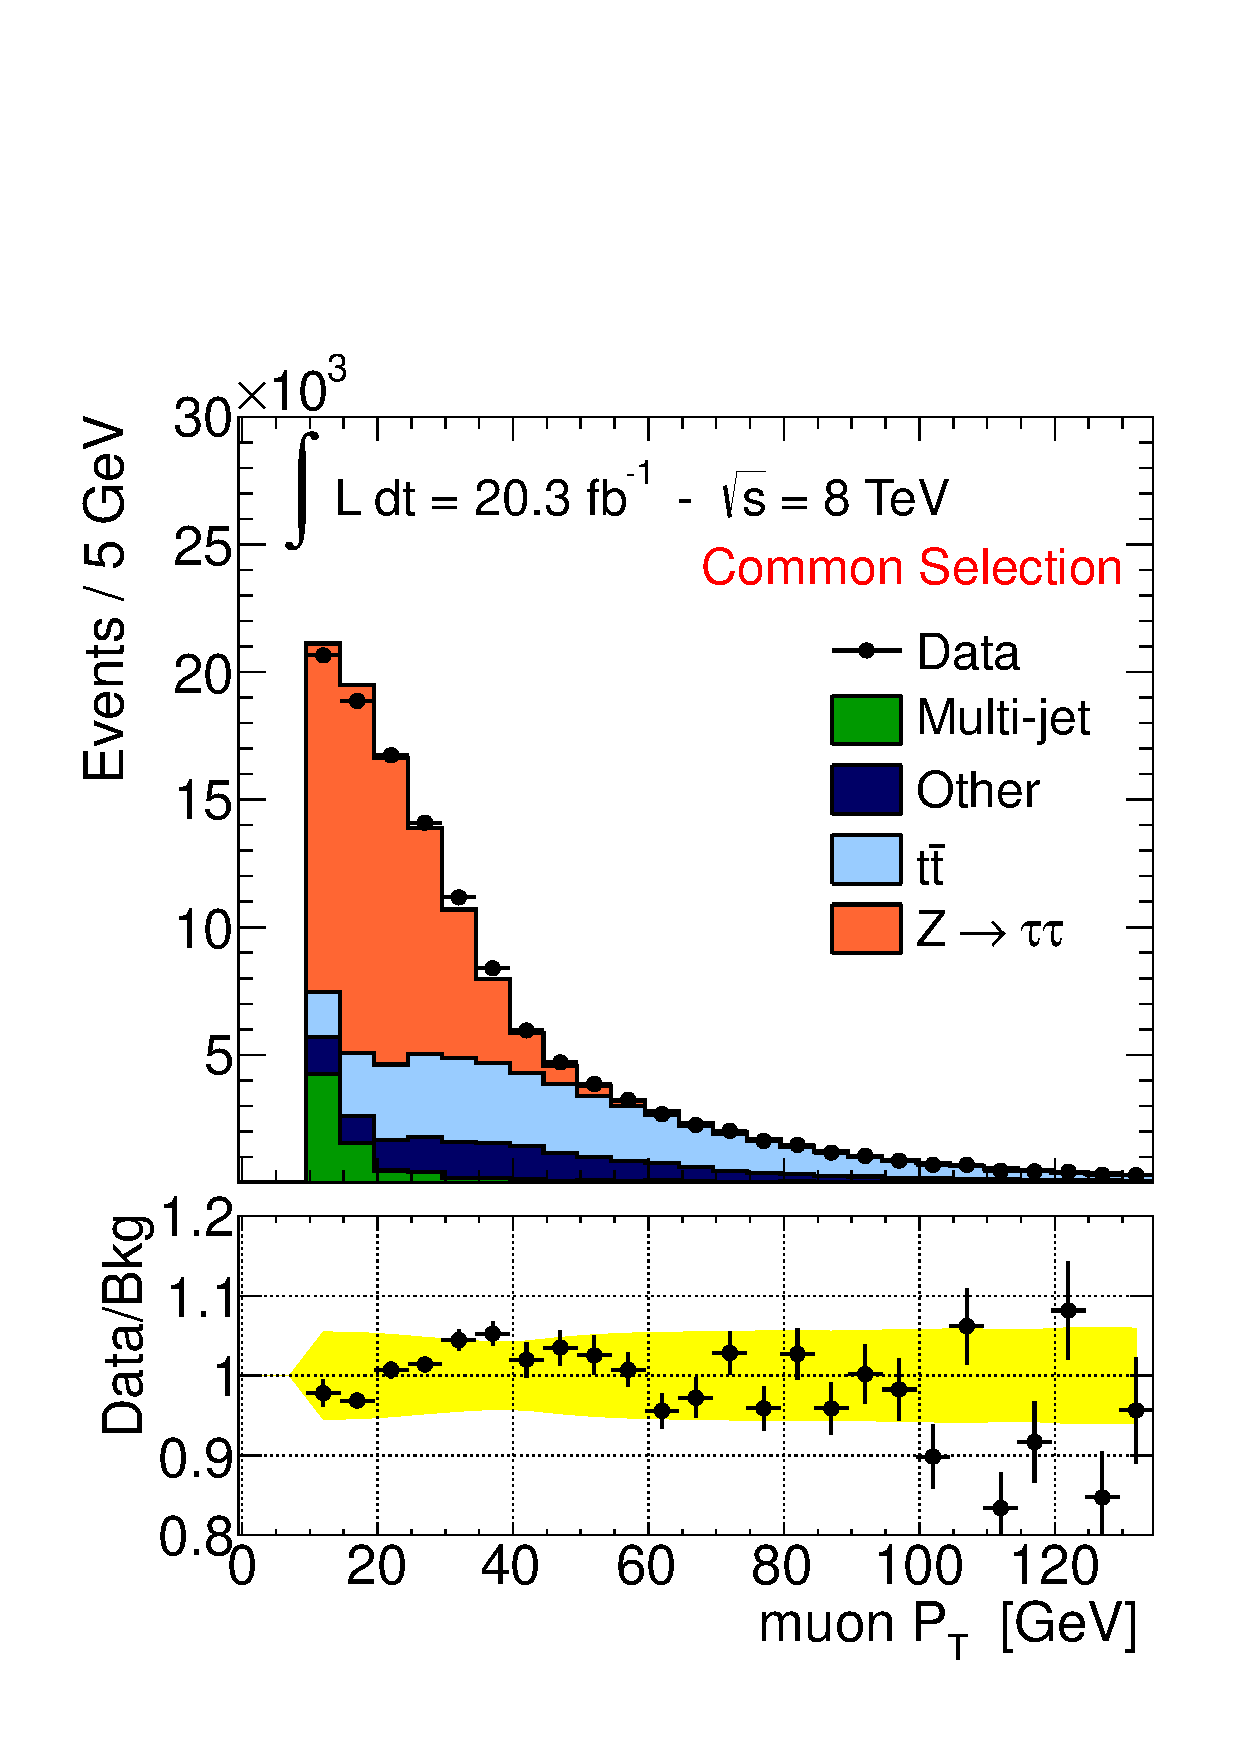
\includegraphics[width=0.47\textwidth]{figure/final_plots/std_presel_muon_pt.pdf}
            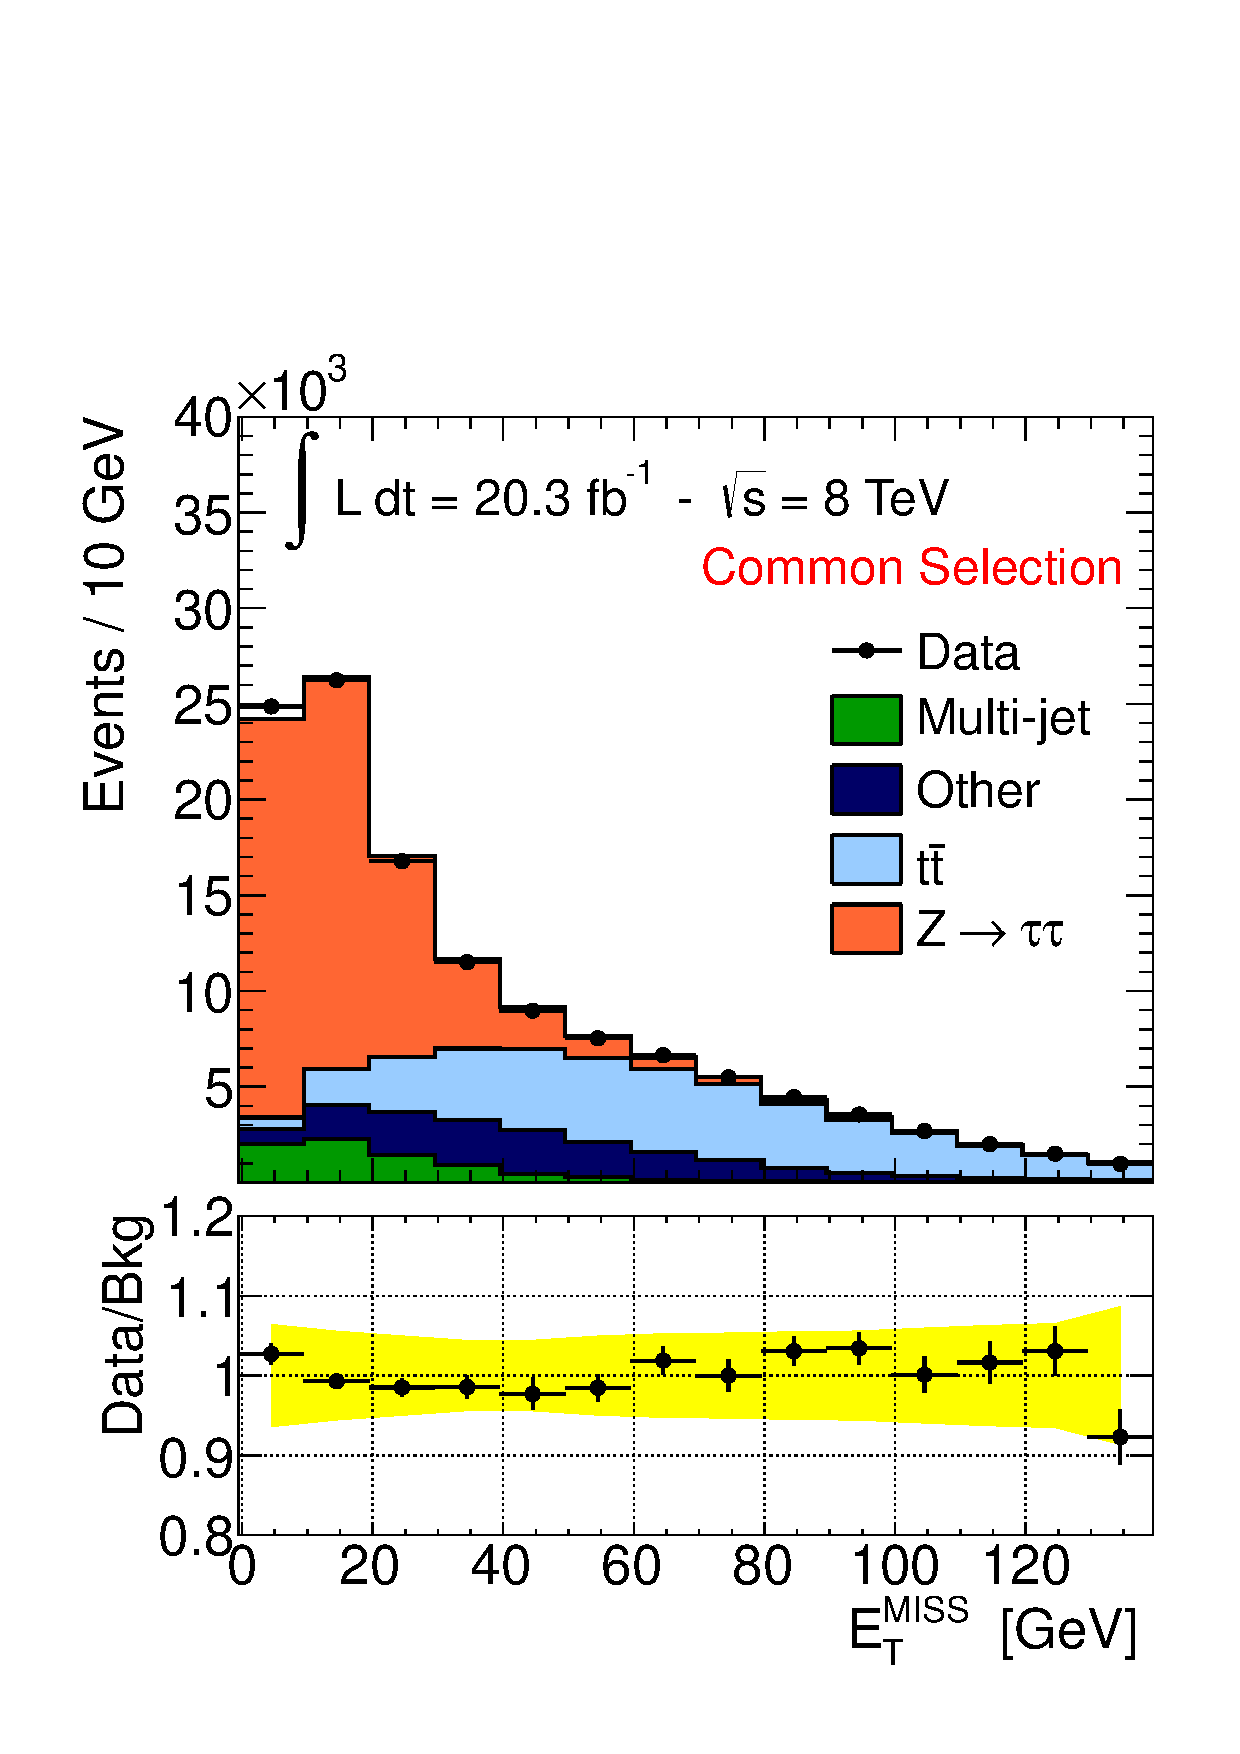
\includegraphics[width=0.47\textwidth]{figure/final_plots/std_presel_EtMiss.pdf}
            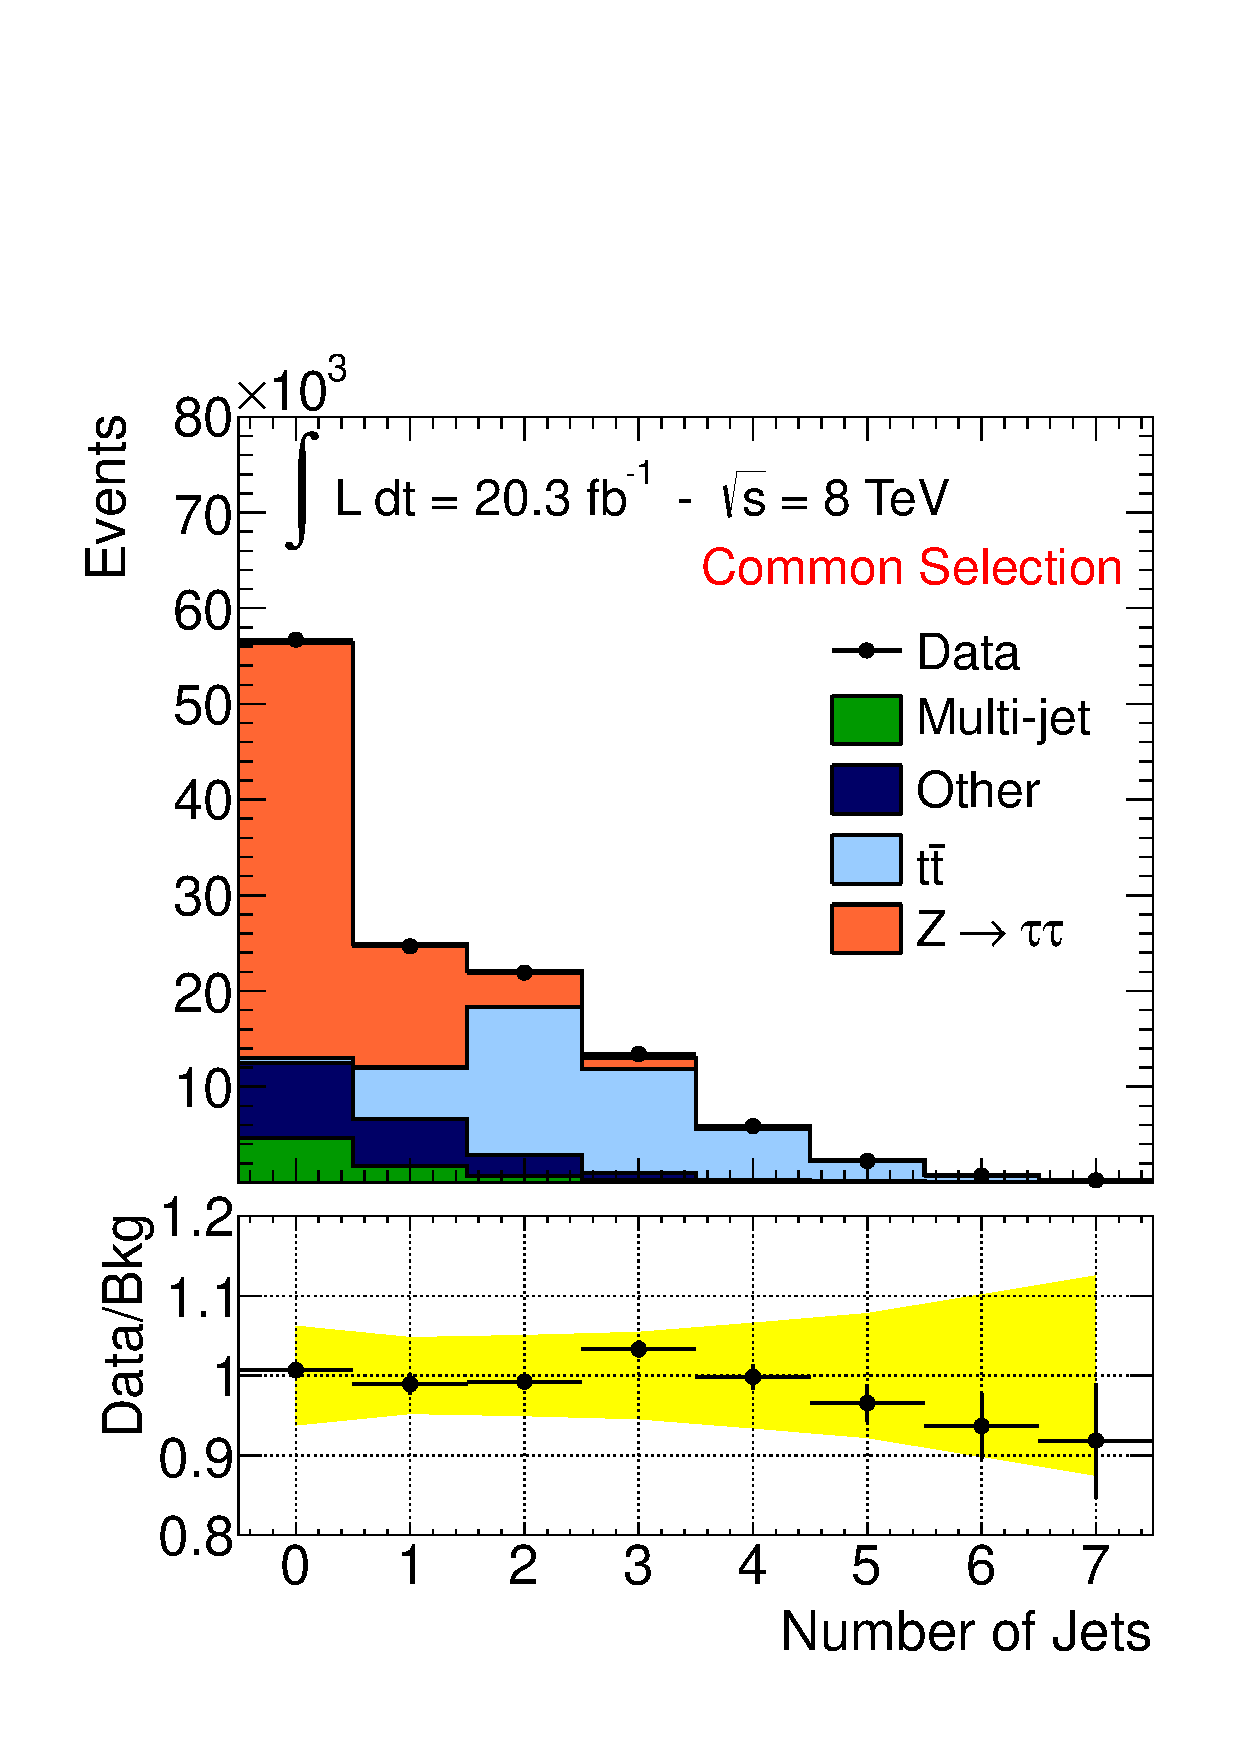
\includegraphics[width=0.47\textwidth]{figure/final_plots/std_presel_nJet_tag.pdf}


    \end{center}
    \caption{ 
	Observed and expected distribution of  kinematic variables after common selections. 
	The prediction of the  background model is compared to  data.
	The contribution of the $\Ztautau$ and QCD multi-jet background processes is measured in  dedicated  signal-depleted control data samples,
	the prediction for all the other bakground processes is obtained from simulation.
 	The notation ``Other'' stands 	for the electroweak processes $\Wlnu$, $\Zll$, diboson and single top quark production.
	The yellow band represents the total systematic uncertainty for the background model prediction.}
   \label{fig:validation}
\end{figure}



\subsection{Validation of the \ttbar Background Prediction}
\label{sec:top_est}

The background contribution from top quark pair production is estimated using a sample of simulated events generated with POWHEG-PYTHIA Monte Carlo
generator. Since this is one of the major background processes for the presented analysis a careful validation 
of the predicted contribution is needed. For this purpose
signal-depleted data validation sample  enriched with \ttbar events  by requiring the presence of exactly two b-tagged jets in all the events
passing the common selection.
%Since this is one of the major backgrounds for this analysis (especially in b-tag category)
%a careful validation of this background model is need, for this purpose a  top quark enriched control region (CR)  
%is defined by adding to the preselection the further requirement of exactly two b-tagged jets in the event. 
Figures~\ref{fig:kinematicsttbar} and~\ref{fig:cutsttbar} show the distributions for a set of kinematic properties and all discriminating 
variables obtained with this  data sample. Good agreement between data and Monte Carlo prediction is found with 
%and shows that our top-quark background model describes well the data
%Also the prediction of the event yield in this CR is in good agreement with data: 
overall ratio of the observed to the predicted number of \ttbar events of $0.998 \pm 0.011\mathrm{(stat.)} \pm 0.110 \mathrm{(sys.)}\,.$
The total systematic uncertainty on the ratio is dominated by the uncertainty of the b-tagging efficiency. 
%In addition, this result could be used
%as a measure of $t\bar{t}$ normalization avoiding systematic uncertainty on the theoretical cross section of
%this process. In this case, however, additional acceptance systematics would need to be evaluated in a dedicated study.
%
%with a dedicated RIVET analysis and uncertainties of the order of the cross section 
%uncertainty are expected, we then drop this possibility considering that wont bring  
%significant improvements.

\begin{figure}[tp]
     \begin{center}

        \subfigure[]{%MMC
            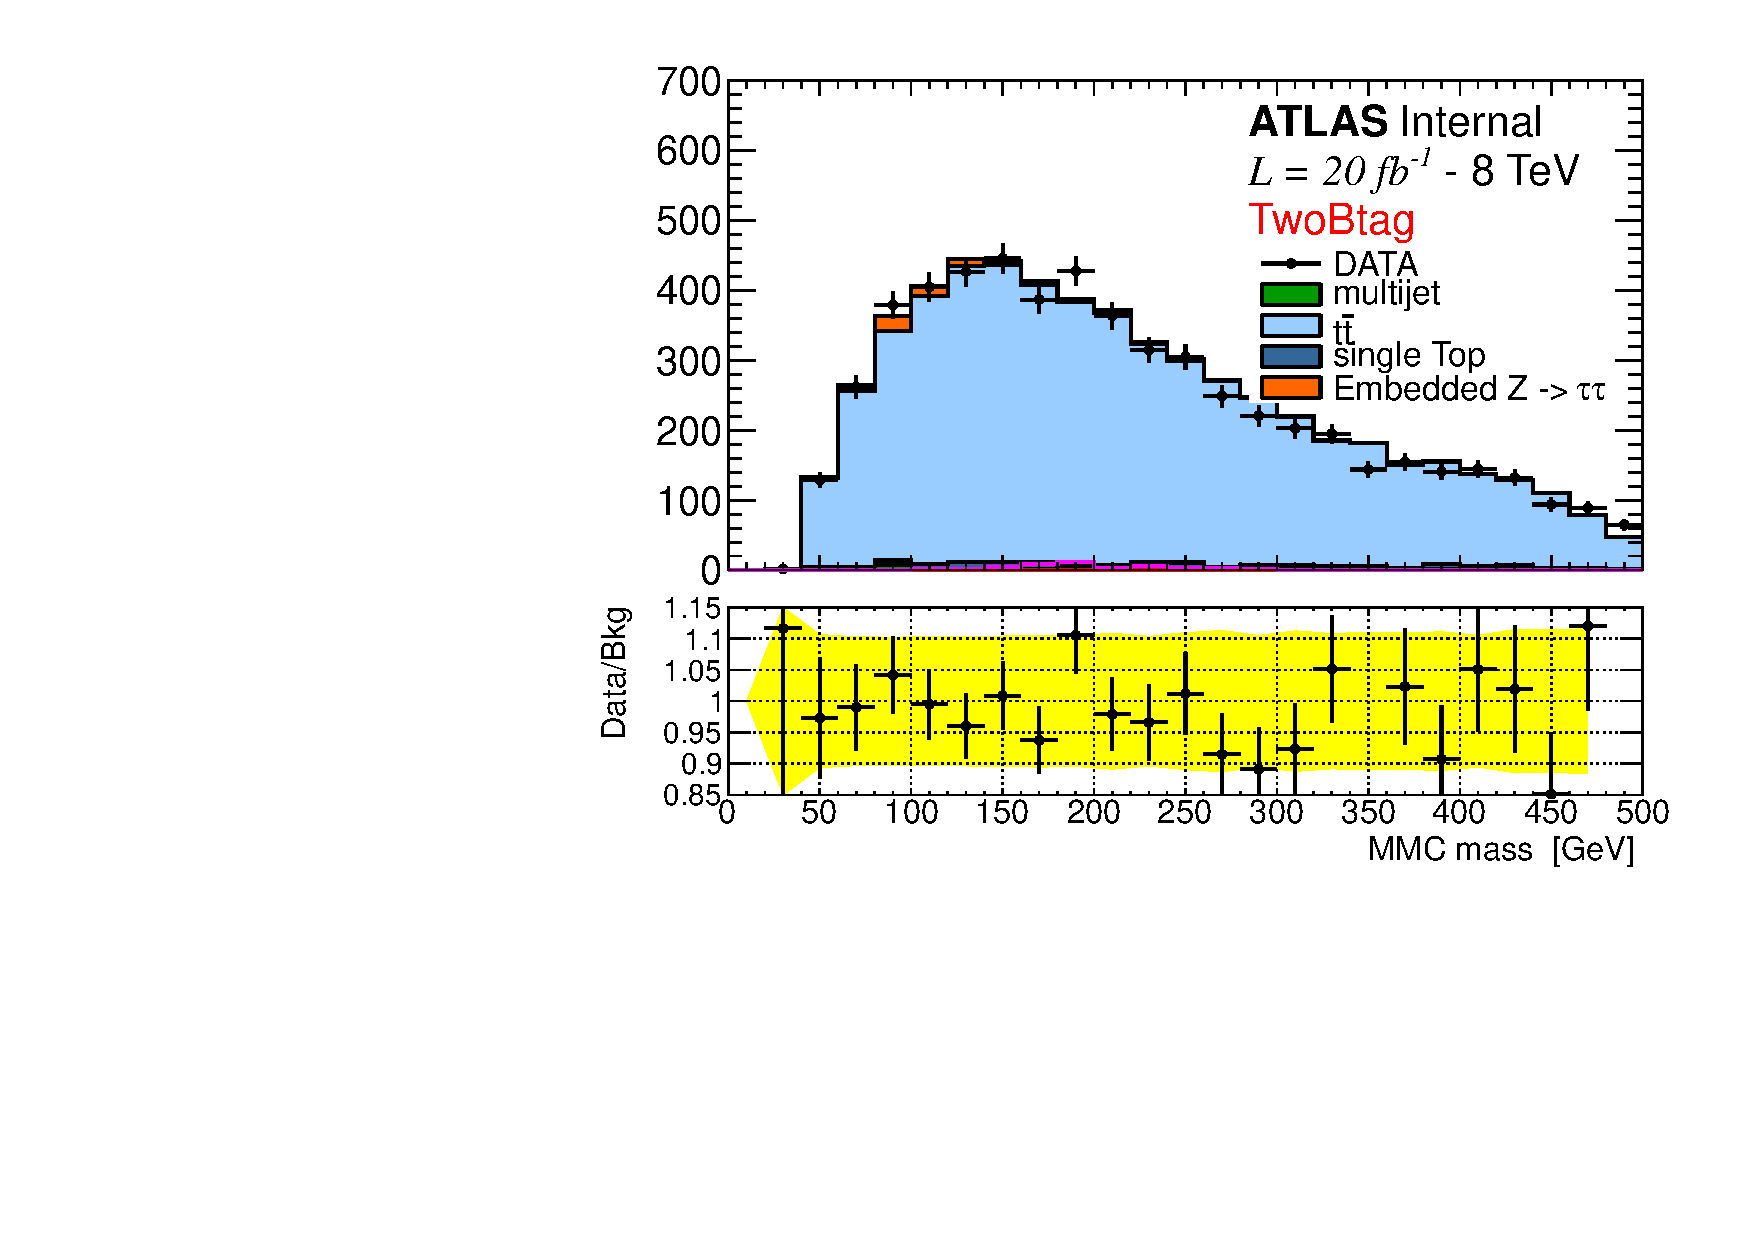
\includegraphics[page=1,width=0.45\textwidth]{figure/bg_estimation/std_plots_twoBtag.pdf}
        }
        \subfigure[]{%ele pT
           \includegraphics[page=6,width=0.45\textwidth]{figure/bg_estimation/std_plots_twoBtag.pdf}
        } 
        \subfigure[]{%Muon pt
            \includegraphics[page=8,width=0.45\textwidth]{figure/bg_estimation/std_plots_twoBtag.pdf}
        }

    \end{center}
    \caption{ Observed and expected distributions  of a) the di-$\tau$ invariant mass
	\mmc, b) the electron transverse momentum $\pt(e)$ and c) the muon transverse momentum $\pt(\mu)$ in the \ttbar validation sample. 
	The error bars on the observed to the predicted events ratio indicates the statistical uncertainty,
	whereas the yellow band indicates the total systematic uncertainty of this ratio.} 
   \label{fig:kinematicsttbar}
\end{figure}


\begin{figure}[ht!]
     \begin{center}

        \subfigure[]{
            \label{fig:cuts_a} %DPhi
            \includegraphics[page=12,width=0.45\textwidth]{figure/bg_estimation/std_plots_twoBtag.pdf}
        }
        \subfigure[]{%CosDphi
            \label{fig:cuts_b}
            \includegraphics[page=13,width=0.45\textwidth]{figure/bg_estimation/std_plots_twoBtag.pdf}
        }\\
        \subfigure[]{%Ht
            \label{fig:cuts_c}
            \includegraphics[page=10,width=0.45\textwidth]{figure/bg_estimation/std_plots_twoBtag.pdf}
        }
        \subfigure[]{%Lep+Et
            \label{fig:cuts_d}
            \includegraphics[page=11,width=0.45\textwidth]{figure/bg_estimation/std_plots_twoBtag.pdf}
        }

    \end{center}
    \caption{ Observed and expected distributions of the discriminating variables, (a) $\Delta\phi(e-\mu)$,
      (b) $\sum\cos\Delta\phi$, (c) \SumLtMET and (d) \Ht  in the \ttbar validation sample.
	The error bars on the observed to the predicted events ratio indicates the statistical uncertainty,
	whereas the yellow band indicates the total systematic uncertainty of this ratio.} 
 
   \label{fig:cutsttbar}
\end{figure}


\subsection{Multi-jet Background Measurement}
\label{sec:qcd}

The QCD multi-jet process represents an important background, 
especially in the b-vetoed event category, due to its high cross-section and the 
relatively low threshold on the lepton \pt used in this analysis. The contribution of this
background is evaluated by the so-called ABCD data-driven technique.
The ABCD method splits the sample of data events after the common selection into four sub-samples: the
signal sample (A), defined by the event selections criteria described in Section~\ref{sec:selection}
and three signal-depleted control data sample (B,C,D), which are orthogonal to each other  and are
enriched in multi-jets events. The three control data samples are defined by inverting the requirements on the relative 
sign of the electron and muon charge  and  on the isolation criteria. 
Both the calorimetric and tracking isolation criteria described in Section~\ref{sec:presel}  are inverted for each electron and muon 
with respect to the nominal values, thus defining the so-called anti-isolated leptons. 
The data are divided into four samples of events with leptons of opposite sign charge (OS) 
or same sign charge (SS) with respectively isolated or anti-isolated leptons, as summarized in Table~\ref{table:qcd}.

\begin{table} [tp]
\centering
\begin{tabular}{c c c }
\hline
Data Sample & Relative Lepton Charge & Lepton Isolation \\ [0.5ex]
\hline
A (signal sample) & OS & isolated \\
\hline
B & SS & isolated \\
C & OS & anti-isolated \\
D & SS & anti-isolated \\ [1ex]
\hline
\end{tabular}
\caption{Control data samples for the measurement of the QCD multi-jet background contribution. The samples are defined by the requirements on the relative
	charge sign of the two leptons (OS,SS) and the isolation criteria applied on them (isolated or anti-isolated). See text.}
\label{table:qcd}
\end{table}

The ABCD method assumes that there is no correlation between the relative 
charge and lepton isolation in QCD multi-jet events, or in other words that the ratio of OS/SS events is uncorrelated 
with the lepton isolation criteria. In this case, the number ($N_{A}$) of QCD multi-jet events in the signal sample $A$ 
can be estimated from the yields ($N_B$, $N_C$, $N_D$)  of multi-jet events in the control samples $B$, $C$ and $D$, using the equation
\begin{equation} \label{eqn:qcdest}
N_{A}  = N_{B} \times \frac{N_{C}}{N_{D}} =  N_{B} \times \rqcd
\end{equation}
%Here is  assumed that the events in the control samples come solely from QCD multi-jet processes, contamination
%from electroweak (W and Z + jets, dibosons) and top processes
%($t\bar{t}$ and single top production) are  subtracted in each control sample 
%using the MC prediction for their event yield.  
To obtain the pure QCD multi-jet event yields in the data control samples, the contribution 
from contaminating electroweak (W+jets, Z+jets and dibosons) and top quark processes
($t\bar{t}$,  single top quark production) is  subtracted in each control sample based 
on the prediction from simulation.
Tables~\ref{table:qcd_yield_btag}~and~\ref{table:qcd_yield_bveto}
show the observed event yield in each control sample at different stages of the event selection along with the
predictions of non-QCD background contributions  which are subtracted.
Signal contamination has been evaluated in all  three control samples for different signal 
mass points. For the range of $m_{A}$ and $\mathrm{tan}\beta$ values considered in this analysis, the highest signal contamination 
is seen in sample B for the mass point $m_{A} = 300$ GeV and $\mathrm{tan}\beta = 50$, where  a contamination 
of 0.2\% is observed\footnote{
This contamination signal originates mainly from the production in association wit b-quarks and,
as it scales with the cross section, it will be an order of magnitude smaller for $\tan\beta = 20\,.$
}.

The modeling of the shapes of kinematic distributions in QCD multi-jet events is given by the data sample B.
The events in this sample are expected to have similar kinematic properties as in  the signal sample.
A drawback of this choice is a rather low number of events and a higher contamination with non-QCD process compared to samples C and D.
Sample B is chosen  to avoid a shape bias due to isolation requirements at the trigger level, since the single-electron trigger 
allready imposes isolation requirements. 
%the trigger:  an isolated trigger is used 
%for electrons (as described in Section~\ref{sec:eventsel}), where the offline requirement equivalent to this trigger choice is $\ptcone20/\pt <0.1$.
Figure~\ref{fig:BvsD} shows the comparison of the electron $\pt$ distributions in sample B and D. In the latter sample 
high-$\pt$ electrons are suppressed as they do not pass the trigger selection. 
Eventually the trigger isolation requirement could also 
bias the ratio \rqcd. This possibility has been carefully studied 
in a dedicated study as reported in Appendix~\ref{appendix:qcd}.
To a good approximation, the mentioned trigger effects cancel out in the ratio
\rqcd and no additional systematic uncertainty needs to be taken into account.


To test the predictions of the ABCD method  an additional validation sample has been defined with the following selection criteria after
applying the common selection:
\begin{itemize}
\item \MET $< 20$ GeV
\item \Ht $< 70$ GeV and \SumLtMET$ < 50$ GeV
\item $0 < \mmc < 80$ GeV  	 
\end{itemize}
This validation sample is designed to enhance the multi-jet background contribution with respect to \Ztautau keeping the final 
state kinematics as similar as possible to the signal sample.
Figure~\ref{fig:ABCD_cr} shows the \mmc distribution for this validation sample with and without the  b-tagging requirements.
Agreement between data and the background predictions is found within statistical and detector-related systematics uncertainty. 

\begin{figure}[tp]
	\begin{center}
	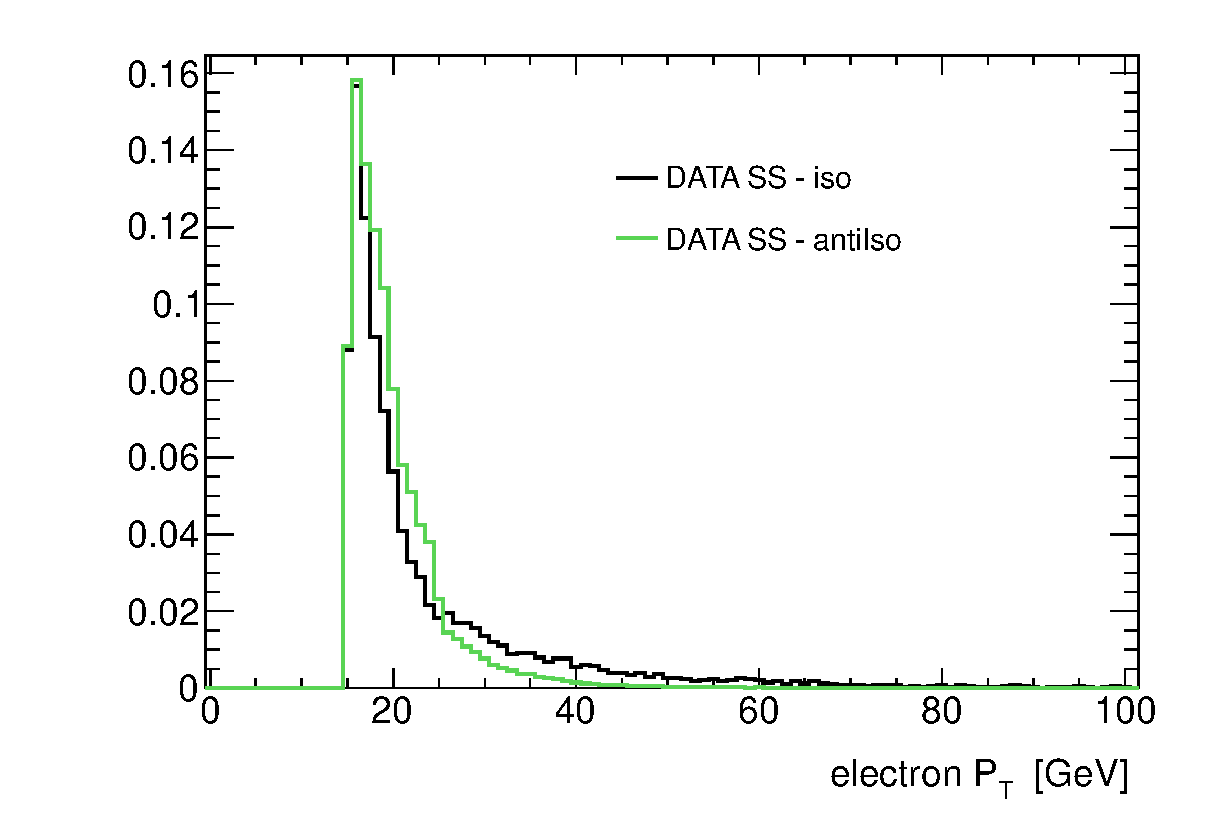
\includegraphics[width=9cm]{figure/ABCD_regionB_Vs_regionD}
	\end{center}
	\caption{Comparison of the electron \pt~distribution in control samples B and sample D, showing the bias due to the trigger. 
	The histograms are normalized to the same area.}
	\label{fig:BvsD}
\end{figure}
%%%%	this table is not that useful

%\begin{table} [p]
%	\caption{Contribution to the different control regions from non-QCD background, after the preselection. }
%	\centering
%	\begin{tabular}{ c c c c c c c}
%%%%%%%%%%%%%%%%%%%%%%%%%%%%%%%%%%%%%%%%%%%%%%%%%%%%%%%%
%\hline
%Region  &  \Ztautau	 & $t\bar{t}$	 & W + jets	 & $Z \rightarrow ll$ + jets & Single Top 	& Dibosons \\ [0.5ex]
%\hline
%  B 	& 341 	$\pm$ 6	&	700$\pm$ 11	&	3398$\pm$ 180	& 830 $\pm$ 58	     &	178$\pm$ 8 		&   612$\pm$ 10  \\
%  C 	& 16 	$\pm$ 2	&	719$\pm$ 12	&	409$\pm$ 50	& 17 $\pm$ 4	     &	103$\pm$ 6		& 13$\pm$ 1 \\
%  D 	& 8	$\pm$ 2	&	539$\pm$ 10	&	49$\pm$	12	& 24$\pm$  7	     &	67$\pm$	 4		& 6$\pm$ 1 \\[1ex]
%\hline
%%%%%%%%%%%%%%%%%%%%%%%%%%%%%%%%%%%%%%%%%%%%%%%%%%%%%%%
%	\end{tabular}
%	\label{table:qcd_mc}
%\end{table}


%%%%%%%%%%%%%%%%%%%%%%%%%%%%%%%%%%%%%%%%%% PUT FINAL NUMBERS!!!!!!!!!!!!!!!! %%%%%%%%%%%%%%%%%%


\begin{table} [p]
	\begin{tabular}[c]{l r c c c c}
%%%%%%%%%%%%%%%%%%%%%%%%%%%%%%%%%%%%%%%%%%%%%%%%%%%%%%%
\hline
\hline 
Event Selection  &  		& B & C & D &  \rqcd \\ 
\hline
Common Selection 	&   Data	&6189			&604628			&312901		    &	1.929 $\pm$  	0.004		\\
	        &   non-QCD	&2510 $\pm$  180  	&1090 $\pm$   30  	&730	$\pm$ 35    &				\\
\hline
B-veto	     	&   Data	&5673		  & 558217 		& 284847		    &	1.960	$\pm$	0.004	\\
	     	&   non-QCD	&2220	$\pm$ 180 & 710 $\pm$ 30	& 415 $\pm$	30	    &				\\
\hline
$\Delta\phi(e-\mu)$  &   Data		&4610		&532583 		&271404		    	    &	1.962	$\pm$	0.005	\\
	     &   non-QCD	&1700 $\pm$170	&580 $\pm$	30	& 345 $\pm$	30	    &				\\
\hline
$\sum\cos\Delta\phi$ &   Data& 3417	&486747 		& 247712	   		    &	1.965	$\pm$	0.005 	\\
	     &   non-QCD     & 1120  $\pm$ 100	& 370 $\pm$ 	20		& 230 $\pm$	20  &				\\
\hline
$\mmc > 0.$    &  Data		& 3177		& 479967 		& 244276	    	    &	1.965	$\pm$	0.005	\\
	     &   non-QCD	& 1000 $\pm$ 100	& 300  $\pm$ 17		&190	$\pm$ 20    &			\\[1ex]
\hline
\hline
%%%%%%%%%%%%%%%%%%%%%%%%%%%%%%%%%%%%%%%%%%%%%%%%%%%%%%%
	\end{tabular}
	\caption{Number of observed events and the predicted non-QCD contribution at different stages of the event selections for b-veto category. 
	The error on the \rqcd ratio is of statistical nature only.}
	\centering
	\label{table:qcd_yield_bveto}
\end{table}

\begin{table} [p]
	\begin{tabular}[c]{l r c c c c}
%%%%%%%%%%%%%%%%%%%%%%%%%%%%%%%%%%%%%%%%%%%%%%%%%%%%%%
\hline 
\hline 
Event Selection  &  		& B & C  & D &  \rqcd \\
\hline
Common Selection&   Data	&6189			&604628			&312901		    &	1.929 $\pm$  	0.004		\\
	        &   non-QCD	&2510 $\pm$  180  	&1090 $\pm$   30  	&730	$\pm$ 35    &				\\
\hline
B-tag	     	&   Data	&419		&44619 			&27257		    &	1.64	$\pm$	0.01	\\
	     	&   non-QCD	&215 $\pm$  10	&310 $\pm$	12	&277 	$\pm$ 13    &				\\
\hline
$\Delta\phi(e-\mu)$  &   Data		&230		&38810 			&23316		    &	1.67	$\pm$	0.01	\\
	     &   non-QCD	&104 $\pm$ 6	&200 $\pm$	10	&175	$\pm$ 7	    &				\\
\hline
$\sum\cos\Delta\phi$ &   Data & 149		&31379 			&18779		    &	1.67	$\pm$	0.02	\\
	     &   non-QCD      & 67 $\pm$ 5	&127 $\pm$	8	&114 $\pm$	6   &				\\
\hline
$\sum H_T$ &   Data	      & 83		& 27781 		&15626		    &	1.78	$\pm$	0.02	\\
	&   non-QCD	      & 23 $\pm$  4	& 25 $\pm$	3	& 22 $\pm$   3	    &				\\ 
\hline
\SumLtMET &   Data	&71		&27735 	&15590		    &	1.78	$\pm$	0.02	\\
	     &   non-QCD	 & 10 $\pm$	3	& 22  $\pm$ 3		&18	$\pm$ 2	    &			\\
\hline
$\mmc > 0.$    &  Data	& 70	& 27634 	& 15522		    			    &	1.78	$\pm$	0.02	\\
	     &   non-QCD	& 9 $\pm$ 3	& 20  $\pm$ 3		&17	$\pm$ 2	    &			\\[1ex]
\hline
\hline
%%%%%%%%%%%%%%%%%%%%%%%%%%%%%%%%%%%%%%%%%%%%%%%%%%%%%%
	\end{tabular}
	\caption{Number of observed events and the predicted non-QCD contribution at different stages of the event selections for b-tag category. 
	The error on the \rqcd ratio is of statistical nature only.}
	\centering
	\label{table:qcd_yield_btag}
\end{table}


\begin{figure}[tp]
	\begin{center}
	     
	\subfigure[]{
		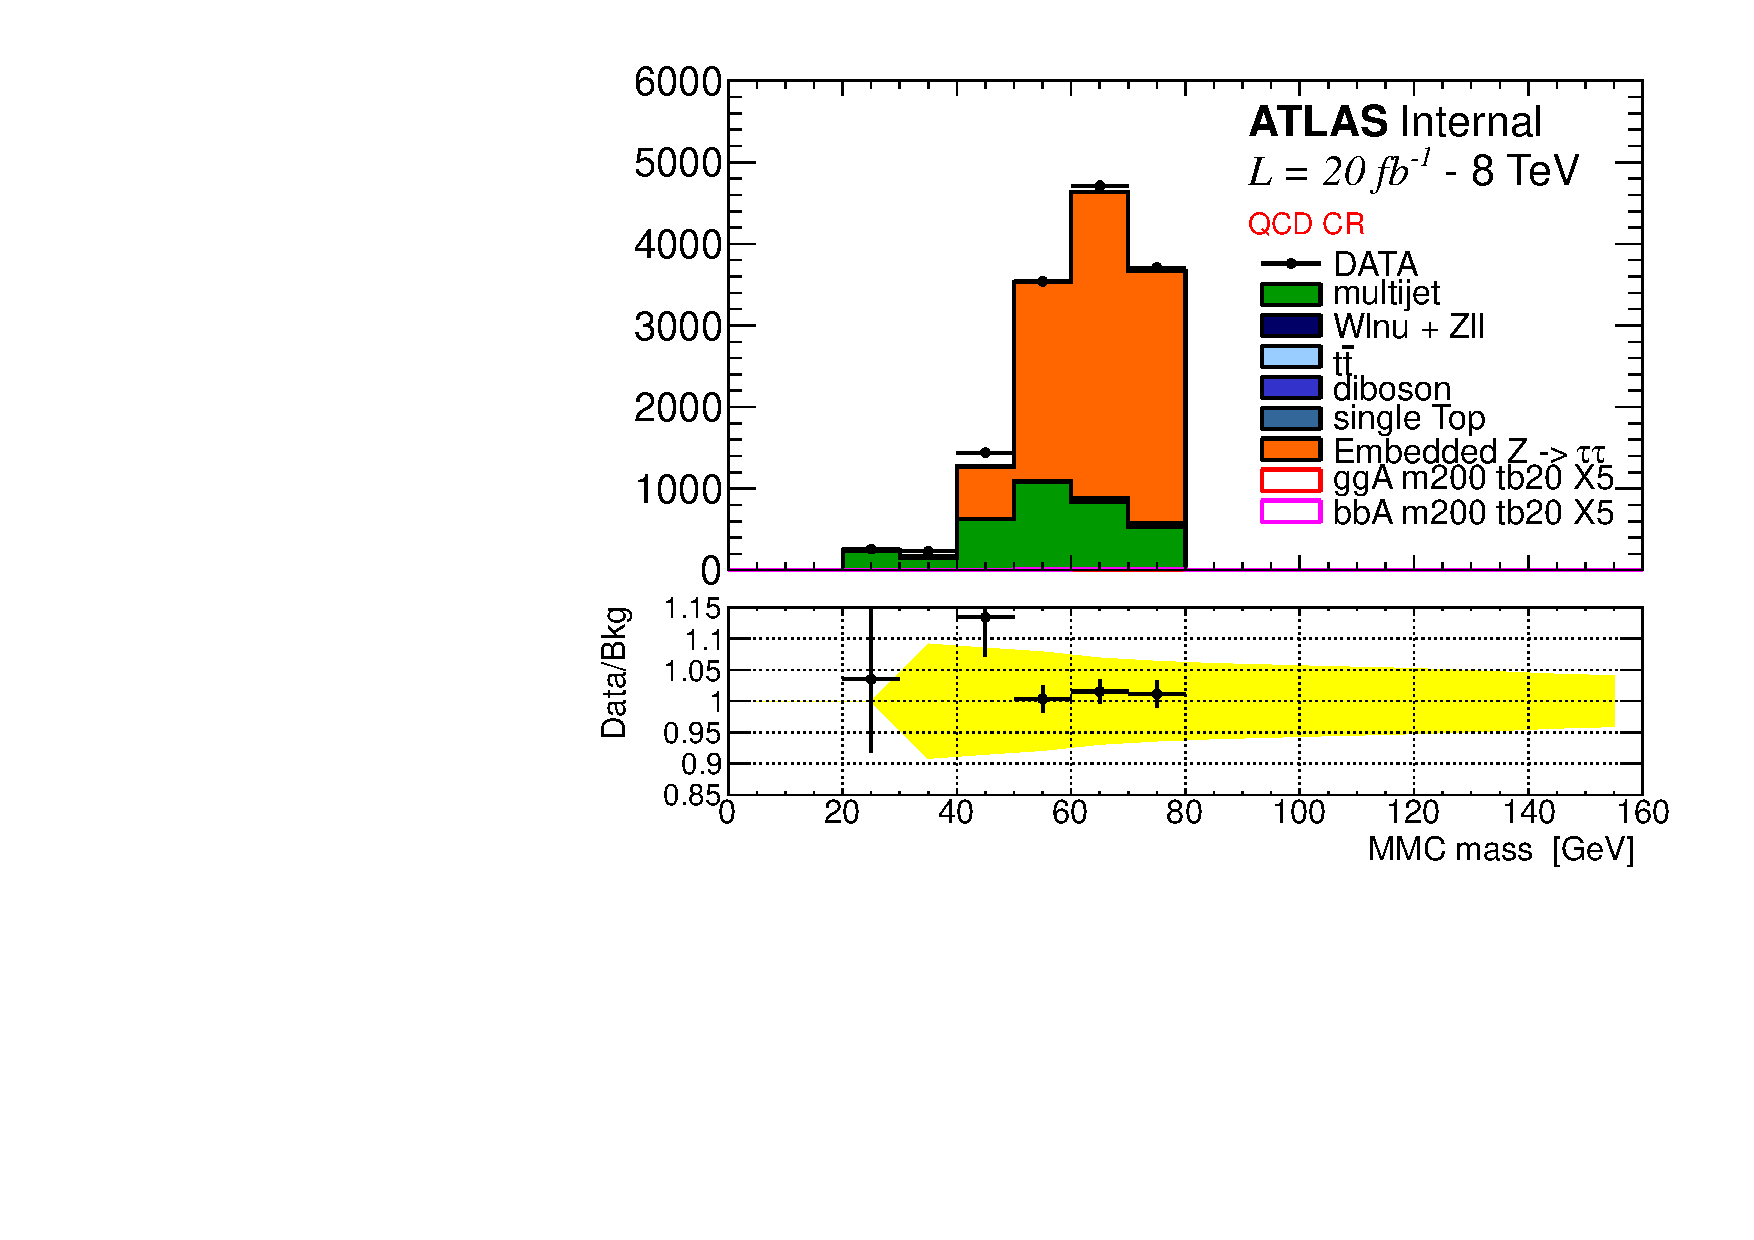
\includegraphics[page=1,width=0.49\textwidth]{figure/QCD/qcd_CR_emb.pdf}
	        }
	\subfigure[]{
  	\includegraphics[page=5, width=0.49\textwidth]{figure/QCD/qcd_CR_emb.pdf}
	}
	
	\end{center}
	\caption{\mmc distribution obtained with QCD validation samples 
	defined in Section~\ref{sec:qcd}, without~(a) and with an additional requirement of exactly one b-tagged jet in the final state~(b).}
	\label{fig:ABCD_cr}
\end{figure}


Systematic uncertainties are assigned on the scaling factor \rqcd and on the shape of
the discriminating variable \mmc to take into account any correlation between the isolation and the relative charge 
of the leptons as detailed in Section~\ref{sec:Systematics}.





\subsection{$Z \rightarrow \tau\tau$ + Jets Background Measurement}\label{sec:ztau}
The  \Ztautau decays are the major source of  background to the presented  analysis,  calling for its thorough understanding.
Unfortunately, for a light Higgs boson, it is impossible to fully discriminate the  \Ztautau decays 
from the signal and thus a 
dedicated signal-free data control sample cannot be defined.
However, thanks to the small Higgs boson coupling to muons, \Zmumu decays provide a good starting point to 
model \Ztautau events based on data. A hybrid approach relying on data and simulation known as the "embedding" is used for this purpose.
The $\Zmumu$ event candidates are selected in data. The two muons from the $Z$ decay are then substituted with the decay 
products from simulated $\tau$ lepton decays. The energy deposit in the calorimeter and the reconstructed tracks 
in a cone of given size around the muon are subtracted
and substituted with the corresponding predictions from the $\tau$ lepton decay. These $\tau$ leptons  have the same kinematic properties
 as the original muons. Further details on the embedding technique may be found in \cite{Embedding, SMold}.

%The selection of the \Zmumu input data requires exactly two combined, opposite charged
%muons, where the leading muon has a transverse momentum $\pt > 20 \GeV$ and 
%the sub-leading muon $\pt > 15\GeV$. Both muons are requited to lie within $|\eta|<2.5$ and to be isolated with 
%$\ptcone 20/\pt<0.2$ (see Section~\ref{sec:presel}). Additionally 
%the invariant mass of the two muons is required to be in the range $M_{\mu\mu} > 40$ GeV.
%Once the muon pair events are selected, all tracks and calorimeter cells associated to the muons are 
%removed from the \Zmumu data event. Finally, the calorimeter cell energy and tracks from the simulated tau decays
%are added to the data event and the event is re-reconstructed.

%A set of corrections are applied to correct for the muon trigger efficiency, the muon reconstruction efficiency and other additional effects
%related to the original \Zmumu events. Finally, as the trigger is not emulated in the embedding sample, 
%an additional correction is applied to emulate the electron and muon trigger efficiencies in the final \Ztautau embedded events. 
%For a full description of the corrections and validation see \cite{SMnew}.

%The embedding technique, which uses \Zmumu decays to 
%model \Ztautau events in a data-driven way, is described in Section~\ref{sec:data_mc}. 
As the Trigger is not simulated in the described embedded samples, only the shapes of kinematic distributions are modelled by the embedded sample,
while the $\Ztt$ event yield
is normalized to ALPGEN \Ztautau prediction at a common selection stage. Furthermore, a set of corrections as described in \cite{SMnew}, is
applied to unfold from the original \Zmumu trigger and reconstruction efficiency. Subsequently,
the trigger and reconstruction efficiency  the $e \mu +4\nu $ final state are emulated by means of event weights.

The embedding technique has been validated in several studies detailed in~\cite{Embedding, SMnew},  demostrating a reliable performance of the embedding technique
and a good description of data. In the context of this analysis, 
Figures~\ref{fig:emb_vs_alp1} and~\ref{fig:emb_vs_alp} show comparisons of various kinematic distributions between
data, embedded and ALPGEN \Ztautau events at the common selection stage. No significant differences are  seen 
between for the \mmc distribution. 
Other relevant discriminating variables, such as the \MET 
and the number of b-jets in the final state, are slightly better described by the embedded $\Ztautau$ sample, as expected due to the 
imperfect modeling of these variables with simulation.

\begin{figure}[tp]
     \begin{center}

            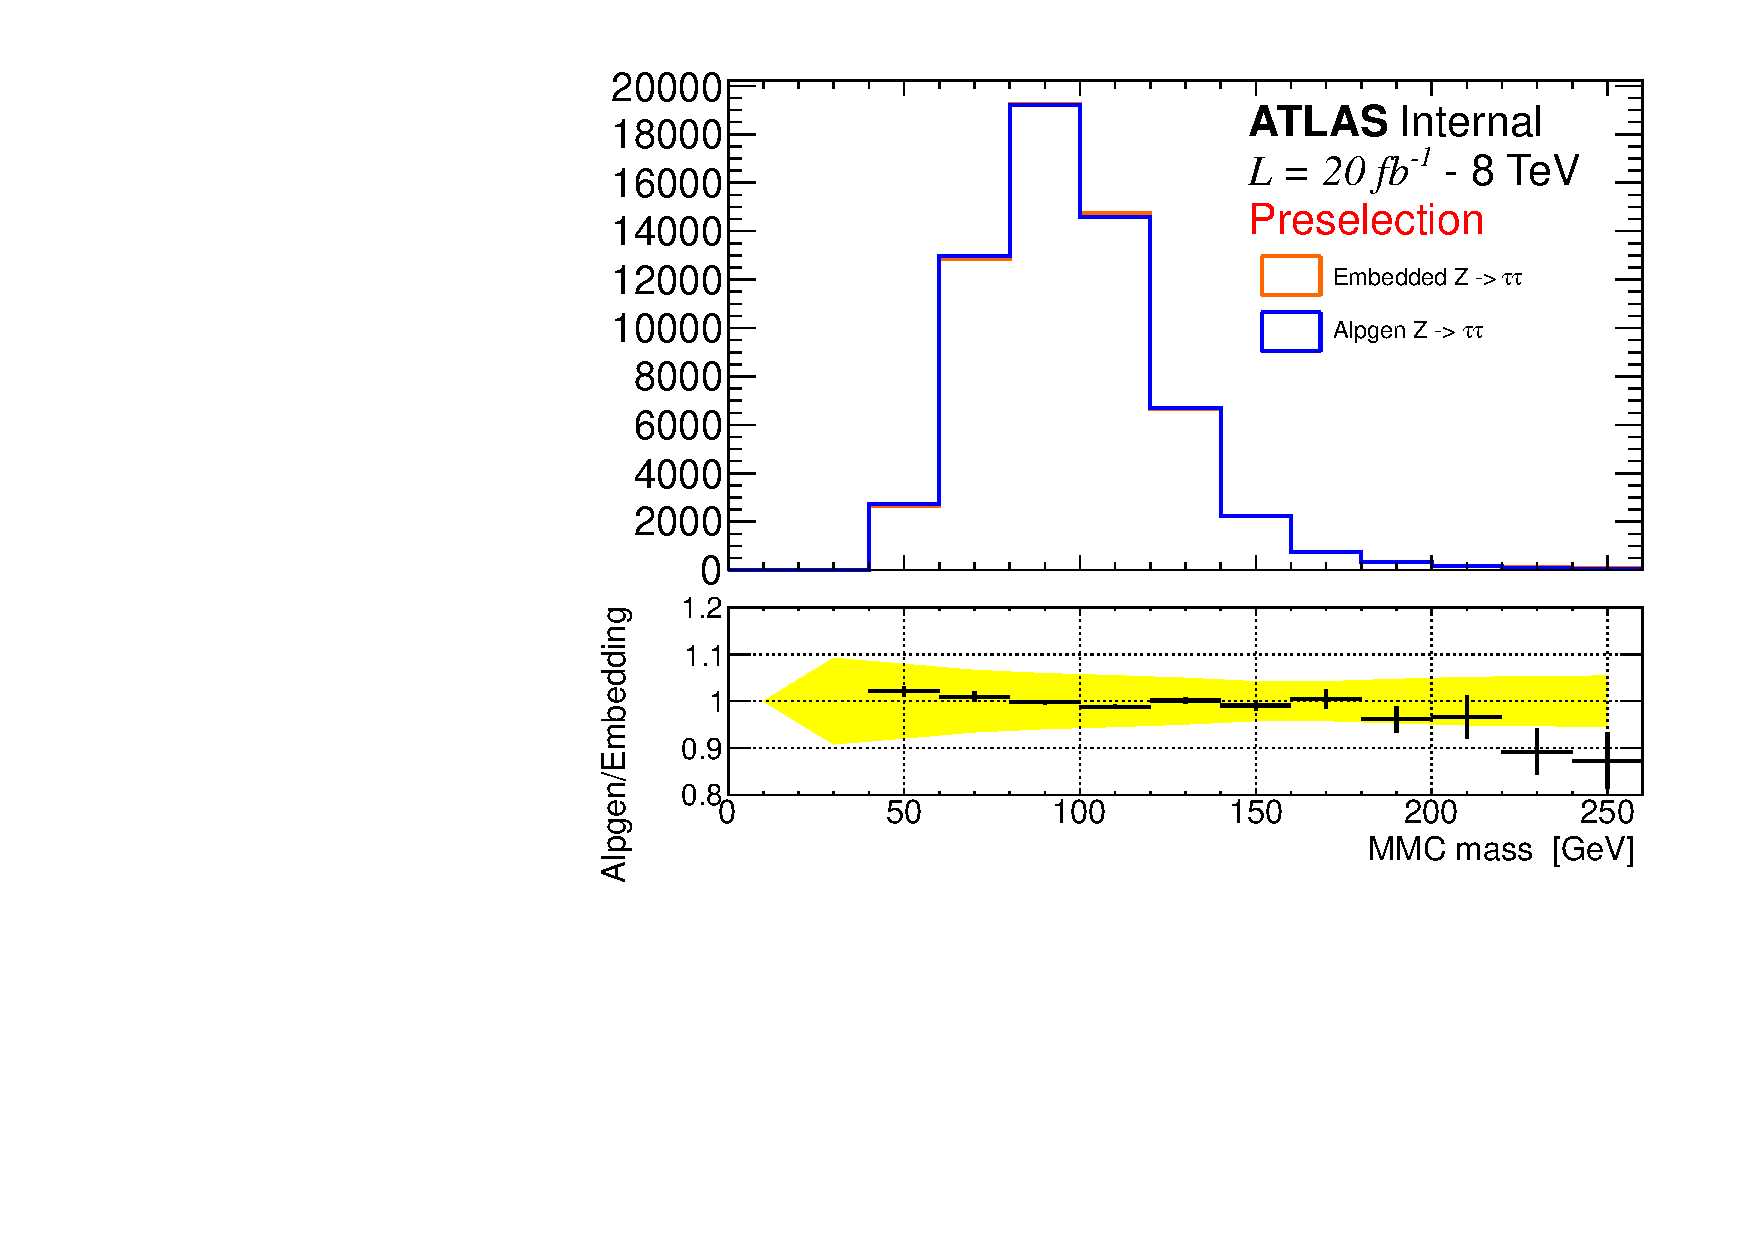
\includegraphics[page=1, width=0.6\textwidth]{figure/bg_estimation/std_plots_emb.pdf}
\end{center}
    \caption{Comparison of the \mmc distributions obtained from the ALPGEN \Ztautau simulation and from the embedding technique after 
	the requirements of th common selection  has been applied. 
	The yellow bad indicates the total systematic uncertainty  relative to the ALPGEN simulation sample.}
   \label{fig:emb_vs_alp1}
\end{figure}


\begin{figure}[tp]
     \begin{center}

           \includegraphics[page=2, width=0.6\textwidth]{figure/bg_estimation/std_plots_emb.pdf}
            \includegraphics[page=3, width=0.6\textwidth]{figure/bg_estimation/std_plots_emb.pdf}

    \end{center}
    \caption{Comparison of the (a)  $\MET$  and (b) b-tagged jet multiplicity distributions in
	embedded and ALPGEN \Ztautau events after the requirements of the common selection has been applied.
	Data are superimposed after subtracting  the contribution of non-\Ztautau processes.The yellow bad indicates
	 the total systematic uncertainty  relative to the ALPGEN simulation sample.}
   \label{fig:emb_vs_alp}
\end{figure}


%plot comparing embedding and ALPGEN Et miss and b-tagging, data -MC not Ztautau and compare data alp and emb.

The embedded sample is based on the selected \Zmumu event candidates in data. The \Zmumu selection criteria 
assure a rather pure \Zmumu sample. However, further event selection criteria used in the presented analysis, 
for example the b-tagging requirements, could enhance the contamination of this sample with events  from other processes. 
Dedicated studies have been made to estimate the $t\bar{t}$ and QCD multi-jet contamination in the embedded sample.
The \ttbar~ contamination is estimated by evaluating the yield of embedded \Ztt events in a validation sample with two b-tagged jets
(as described in Section~\ref{sec:top_est}). These events are assumed to originate solely from the $t\bar{t}$ process
and the corresponding yield in the signal sample is extrapolated from simulation.
Table~\ref{table:emb_cont_tt} summarizes the evaluated top quark contamination in the embedded $\Ztt$ sample, separately for the two event categories.
The multi-jet contamination can be estimated starting 
from the yield of embedded events in the sample C defined by the ABCD method.
%one should not use SS samples because embedding already requires leptons to be OS, then would be biased
It is assumed that all events in this validation sample are QCD multi-jet events. The QCD multi-jet contamination 
of the embedded events in the  signal sample 
can be estimated as:
\begin{equation} \label{eqn:qcdEmb}
N_{A}^{QCD-emb}  = N_{C}^{QCD-emb} \times \frac{N_{B}^{\mu\mu}}{N_{D}^{\mu\mu}} =  N_{B} \times R_{QCD}^{\mu\mu}
\end{equation}
The transfer factor $R_{QCD}^{\mu\mu}$, is evaluated using a di-muon final state with same kinematic selection criteria
 as for \Zmumu candidates entering the embedding procedure.
Table~\ref{table:emb_cont_qcd} shows the estimated contamination of QCD multi-jet in the embedded sample.  
Contamination effects are considered negligible.


\begin{table} [tp]
\begin{small}
\centering
\begin{tabular}{c c c c c}
\hline
\hline
 & Yield of 		& Transfer	& Estimated events	& Contamination \\
 & embedded events	& factor	& in signal sample	&	\\		 [0.5ex]
\hline
b-tag & $84 \pm 9$  & $(2.6 \pm 0.1) \times 10^{-2}$ &  $2.2 \pm 0.2$&  0.5 \% \\
b-veto & $84 \pm 9$ & $(1.74 \pm 0.02) \times 10^{-1}$ & $15 \pm 2$ & 0.03 \% \\[1ex]
\hline
\end{tabular}
\end{small}
\caption{Evaluation of the $t\bar{t}$ contamination  in the embedded $\Ztt$ sample using a two b-tag validation sample. 
The transfer factor is a multiplicative factor obtained from simulation that allows to extrapolate
the measuremet from the validation sample into the signal sample. }
\label{table:emb_cont_tt}
\end{table}

\begin{table} [tp]
\begin{small}
\centering
\begin{tabular}{c c c c c}
\hline
\hline
 & Yield of embedded events	& Transfer	& Estimated events	& Contamination \\
 &  in QCD control sample C		& factor	& in signal sample	&	\\		 [0.5ex]
\hline
B-tag  & $12 \pm 3$ & $ (7 \pm 1) \times 10^{-3}$ &  $(8.4 \pm 0.3) \times 10^{-2}$ &  0.03 \% \\
B-veto & $390 \pm 20$ & $(2.5 \pm 0.1) \times 10^{-2}$ & $10.0 \pm 0.5$ & 0.02 \% \\[1ex]
\hline
\end{tabular}
\end{small}
\caption{Evaluation of the QCD multi-jet contamination  in the embedded $\Ztt$ sample  using the control sample
 with OS anti-isolated events (sample C). The transfer factor $R_{QCD}^{\mu\mu}$ is the
multiplicative factor that allows to extrapolate the measured events in control sample C into the signal sample.
The transfer factor is evaluated using di-muon events with same kinematic properties as the  $\Zmumu$ candidates 
entering the embedding procedure.}
\label{table:emb_cont_qcd}
\end{table}



